\subsection{Our GPU-based Static PageRank}
\label{sec:static}

We first discuss our GPU implementation of Static PageRank. Its psuedocode is given in Algorithm \ref{alg:static}. The explanation of the psuedocode is given in Section \ref{sec:static-impl}.

\paragraph{Copying data to the device:}

We begin by copying the CSR representation of the transpose of the current graph $G^{t'}$ to the GPU.

\paragraph{Partitioning vertices into low-degree and high-degree sets:}

We employ a pair of kernels, namely a thread-per-vertex kernel and a block-per-vertex kernel, for rank computation on the GPU. For this, we partition the vertex IDs for the two kernels by their in-degree. The thread-per-vertex kernel handles vertices with low in-degrees, while the block-per-vertex kernel computes ranks of high in-degree vertices. Using two different kernels allows us to improve processing performance for high-degree vertices, while minimizing thread divergence for low-degree vertices. The psuedocode for partitioning\ignore{vertex IDs} is given in Algorithm \ref{alg:partition}, and is explained in Section \ref{sec:partition}.

\paragraph{Rank computation of each vertex:}

We find that, unlike on multicore CPUs, employing a synchronous implementation of the PageRank algorithm, utilizing two separate rank vectors, yields superior performance. Consequently, we opt for a \textit{synchronous} implementation of the PageRank algorithm. During the rank computation phase in each iteration, we employ two distinct kernels. The \textit{thread-per-vertex} kernel manages vertices with low in-degree, assigning one thread per vertex to independently update each vertex's rank in a sequential manner. Conversely, the \textit{block-per-vertex} kernel allocates a thread block per vertex. Within each thread block, threads compute the rank contribution of in-neighbors to the vertex in a strided manner. These partial rank contributions are stored in shared memory, and a block reduction (summation) operation is performed to obtain the net rank contribution. Subsequently, the first thread in the thread block updates the rank of the\ignore{respective} vertex.\ignore{To ensure efficient workload distribution, the vertex IDs between the two kernels are partitioned based on in-degree. This strategy ensures that the workload assigned to each thread is proportional to the in-degree of its corresponding vertex during the rank computation phase, thereby minimizing thread divergence.}

\ignore{We observe that, unlike on multicore CPUs, a synchronous implementation of the PageRank algorithm, which uses two separate rank vectors offers better performance than an asynchronous approach (which performs well on multicore CPUs). Accordingly, we use a \textit{synchronous} implementation of the PageRank algorithm. For the rank computation phase in each iteration, we use two different kernels --- a thread-per-vertex kernel for processing vertices with low in-degree, and a block-per-vertex kernel for processing high in-degree vertices. The \textit{thread-per-vertex} kernel schedules one thread per vertex, and updated the rank of each vertex independently (in a sequential manner). On the other hand, the \textit{block-per-vertex} kernels schedules a thread block per vertex, where each thread in a thread block computes the rank contribution of in-neighbors to the vertex in a strided fashion. These partial rank contributions are the written to shared memory, and a block reduce (sum) is performed to obtained the net rank contribution. The first thread in the thread block then updates rank of the given vertex. The vertex IDs between the two kernels are partitioned by in-degree (the work to be performed by each thread is proportional to the in-degree of each vertex during the rank computation phase), and hence, the thread divergence is expected to be minimal.}

\paragraph{Convergence detection:}

To determine if the ranks of vertices have converged, we calculate the $L_\infty$-norm of the difference between the current and previous ranks. If this value is below the specified iteration tolerance $\tau$, the algorithm terminates, indicating convergence. If not, we swap the current and previous ranks and proceed to the next iteration. The calculation of the $L_\infty$-norm involves two kernels. The first kernel computes the $L_\infty$-norm of the rank differences for each thread block in a grid and stores the results in a temporary buffer. The second kernel computes the net $L_\infty$-norm of the results in the buffer, which is then transferred to the CPU.




\subsection{Our Static PageRank implementation}
\label{sec:static-impl}

Algorithm \ref{alg:static} outlines the psuedocode of our GPU-based Static PageRank. It takes as input the transpose of the current graph snapshot $G^{t'}$, and returns the computed rank vector $R$.

The algorithm begins by initializing the rank vectors $R$ and $R_{new}$, where each vertex's initial rank is set to $1/|V^{t'}|$ (lines \ref{alg:static--initialize-begin}-\ref{alg:static--initialize-end}). We then partition the vertex IDs in $P'$ based on their in-degree (line \ref{alg:static--partition}). This partitioning step is crucial for efficient computation on the GPU. Next, in lines \ref{alg:static--compute-begin}-\ref{alg:static--compute-end}, PageRank iterations are performed. Within each iteration, the ranks are updated using the \texttt{updateRanks()} function (line \ref{alg:static--update}), which computes the updated PageRank scores $R_{new}$ for each vertex based on the previous iteration's ranks $R$ (synchronous). When invoking \texttt{updateRanks()}, we disable the use of vertex and neighbor affected flags ($\delta_V$ and $\delta_N$) in order the utilize the same function for Static PageRank (\texttt{updateRanks()} is also used with DF-P PageRank). After updating the ranks, we calculate the $L_\infty$-norm difference $\Delta R$ between the current $R_{new}$ and previous ranks $R$ to check for convergence (line \ref{alg:static--error}). If the change in ranks falls below the specified tolerance $\tau$, the algorithm terminates (line \ref{alg:static--converged}). Finally, the algorithm returns the converged rank vector $R$ (line \ref{alg:static--return}).

Algorithm \ref{alg:static} uses a pull-based approach for PageRank computation, where each vertex's rank is updated through a single write by a thread. This is in contrast to a push-based approach, where each thread calculates and sums the outgoing PageRank contribution of its vertex to its neighbors, necessitating atomic updates \cite{verstraaten2015quantifying}. We find this to be more efficient and employ it for all implementations \cite{sahu2024df}. We also employ an synchronous implementation of Static PageRank, using two separate rank vectors, which we observe to perform better than an asynchronous implementation.

\begin{algorithm}[!hbt]
\caption{Our GPU-based Static PageRank.}
\label{alg:static}
\begin{algorithmic}[1]
\Require{$G^{t'}(V^{t'}, E^{t'})$: Transpose of current input graph}
\Require{$R, R_{new}$: Rank vector in the previous, current iteration}
\Ensure{$P'$: Partitioned vertex IDs, low in-degree first }
\Ensure{$N'_P$: Number of vertices with low in-degree}
\Ensure{$\Delta R$: $L\infty$-norm between previous and current ranks}
\Ensure{$\tau$: Iteration tolerance}

\Statex

\Function{static}{$G^{t'}$}
  \State $\rhd$ Initialize ranks
  \State $R \gets R_{new} \gets \{\}$ \label{alg:static--initialize-begin}
  \ForAll{$v \in V^{t'}$ \textbf{in parallel}}
    \State $R[v] \gets R_{new}[v] \gets 1/|V^{t'}|$
  \EndFor \label{alg:static--initialize-end}
  \State $\rhd$ Partition vertex IDs by in-degree 
  \State $\{P', N'_P\} \gets partition(G^{t'})$ \label{alg:static--partition} \Comment{Alg. \ref{alg:partition}}
  \State $\rhd$ Perform PageRank iterations
  \ForAll{$i \in [0 .. MAX\_ITERATIONS)$} \label{alg:static--compute-begin}
    \State $updateRanks(\cdots, \cdots, R_{new}, R, G^{t'}, P', N'_P)$ \Comment{Alg. \ref{alg:update}} \label{alg:static--update}
    \State $\Delta R \gets l_{\infty}NormDelta(R_{new}, R)$ \textbf{;} $swap(R_{new}, R)$ \label{alg:static--error}
    \If{$\Delta R \leq \tau$} \textbf{break} \label{alg:static--converged}
    \EndIf
  \EndFor \label{alg:static--compute-end}
  \State \ReturnInline{$R$} \label{alg:static--return}
\EndFunction
\end{algorithmic}
\end{algorithm}





\subsection{Our GPU-based Dynamic Frontier with Pruning (DF-P) PageRank}
\label{sec:frontier}

When dealing with a batch update comprising edge deletions $(u, v) \in \Delta^{t-}$ and insertions $(u, v) \in \Delta^{t+}$, if the total update size $|\Delta^{t-} \cup \Delta^{t+}|$ is relatively small compared to the total edge count $|E|$, only a small fraction of vertices are expected to undergo rank changes. To handle this, our earlier work proposed \textbf{Dynamic Frontier (DF)} and \textbf{Dynamic Frontier with Pruning (DF-P)} approaches, which employ an incremental process to identify affected vertices and update their ranks. Our research showed that DF/DF-P PageRank outperformed Static and Dynamic Traversal (DT) PageRank by $5.2\times$/$15.2\times$ and $1.3\times$/$3.5\times$\ignore{respectively} on real-world dynamic graphs, and by $7.2\times$/$9.6\times$ and $4.0\times$/$5.6\times$ on large graphs with random batch updates \cite{sahu2024df}.

Unfortunately, multicore CPUs have limited memory bandwidth and parallelism, making them unsuitable for graph algorithms like PageRank, which have a low computation-to-communication ratio. In contrast, GPUs offer high-bandwidth memory, connected in close proximity to thousands of lightweight cores with user-managed caches. Moreover, GPU hardware is designed to switch running threads at no cost to support memory access latency hiding. When appropriately designed, graph algorithms can significantly outperform CPU-based implementations on GPUs. This makes a GPU implementation of DF and DF-P PageRank attractive. In this section, we describe the design of DF and DF-P PageRank for GPUs.

\paragraph{Copying data to the device:}

\ignore{A GPU has its own memory that supports a high volume of data transfers.}We\ignore{first} copy the CSR representation of the current graph $G^t$, its transpose $G^{t'}$, the previous ranks of each vertex $R^{t-1}$, and the batch update consisting of edge deletions $\Delta^{t-}$ (both source and target vertex IDs in separate arrays) and edge insertions $\Delta^{t+}$ (source vertex IDs only) to the global memory of the GPU. The CSR of $G^{t'}$ is used for computing PageRank scores, while that of $G^t$ is used for the initial and incremental marking of affected vertices. Note that we only need the source vertex IDs of edge insertions $(u, v) \in \Delta^{t+}$ as we only need to mark the outgoing neighbors of $u$ as affected. On the other hand, for edge deletions $(u, v) \in \Delta^{t-}$, we need both the source and target vertex IDs as we need to mark both the outgoing neighbors of $u$ and the target vertices of the edge deletions, i.e., $v$, as affected.

\paragraph{Partitioning vertices into low-degree and high-degree sets:}

The work to be performed by each thread is proportional to the in-degree of each vertex during the rank computation, and to the out-degree of each vertex during incremental marking of affected vertices. Thus, similar to Static PageRank, we use a pair of kernels, i.e., a \textit{thread-per-vertex} kernel and a \textit{block-per-vertex} kernel, for both the rank computation and the incremental marking phases, by partitioning the vertex IDs for the two kernels by their in-degree for the rank computation phase, and by their out-degree for the incremental marking phase. This also helps minimize thread divergence with the thread-per-vertex kernel. The psuedocode for partitioning the vertices (by in- or out-degree of vertices) is given in Algorithm \ref{alg:partition}, with its explanation given in Section \ref{sec:partition}.

\paragraph{Marking the initial set of affected vertices:}

Upon each edge deletion $(u, v) \in \Delta^{t-}$ and insertion $(u, v) \in \Delta^{t+}$ in the batch update, with the DF and DF-P approaches, we need to mark the outgoing neighbors of vertex $u$ in both the previous $G^{t-1}$ and current graph $G^t$ as affected. This is equivalent to marking the outgoing neighbors of the source vertex, $u$, for each edge deletion and insertion $(u, v) \in \Delta^{t-} \cup \Delta^{t+}$, and marking the target vertex, $v$, of each edge deletion $(u, v) \in \Delta^{t-}$ as affected. We use one kernel to mark the target vertex, $v$, for each edge deletion $(u, v) \in \Delta^{t-}$ as affected, and use a temporary array to indicate that the outgoing neighbors of the source vertex, $u$, for each edge deletion and insertion $(u, v) \in \Delta^{t-} \cup \Delta^{t+}$ need to be marked as affected later. A thread-per-vertex kernel and block-per-vertex kernel are then used to actually mark the outgoing neighbors of such vertices as affected. The vertex IDs between the two kernels are partitioned by out-degree, as mentioned above.

\paragraph{Rank computation and incremental expansion / contraction of the set of affected vertices:}

Similar to our Static PageRank, we adopt a synchronous implementation of the PageRank algorithm, employing a kernel pair during each iteration's rank computation phase. In addition, with the DF and DF-P approaches, if the relative change in the rank of a vertex $u$ is greater than the frontier tolerance $\tau_f$, we need to incrementally mark the outgoing neighbors $v \in G^t.out(u)$ of $u$ as affected \cite{sahu2024df}. However, performing this incremental marking during the rank computation phase may introduce significant thread divergence (the work is proportional to the out-degree of $u$, and not its in-degree). To avoid this, we use a temporary array to indicate that the neighbors of $u$ need to be incrementally marked as affected. This can later be used with a pair of kernels to actually mark the outgoing neighbors of such vertices as affected.

With the DF-P approach, if the relative change in the rank of a vertex $u$ falls within the prune tolerance $\tau_p$, the vertex $u$ needs to be marked as not affected \cite{sahu2024df}. This is achieved by directly unflagging it in the set of affected vertices, which entails $O(1)$ work and does not introduce significant thread divergence. Additionally, considering the potential pruning of vertices and the incorporation of a self-loop for each vertex in the graph (as discussed in Sections \ref{sec:dataset} and \ref{sec:batch-generation}), we employ a closed-loop formula for computing the rank of each vertex (Equation \ref{eq:pr-prune}). This formula is specifically designed to accommodate the presence of the self-loop, thereby mitigating the need for recursive rank calculations stemming from it \cite{sahu2024df}. We refer the reader to our prior work \cite{sahu2024df} for an example of the DF and DF-P approaches.

\paragraph{Convergence detection:}

This is similar to that of Static PageRank.

\begin{flalign}
\label{eq:pr-prune}
  R[v] & = \frac{1}{1 - \alpha / |G.out(v)|} \left(\alpha K + \frac{1 - \alpha}{|V|}\right) && \\
    \text{where, } K & = \left(\sum_{u \in G.in(v)} \frac{R[u]}{|G.out(u)|}\right) - \frac{R[v]}{|G.out(v)|}
\end{flalign}


\ignore{\subsubsection{A simple example}}

\ignore{Figure \ref{fig:about-frontier} provides an illustration of DF and DF-P PageRank. Initially, as demonstrated in Figures \ref{fig:about-frontier-df1} and \ref{fig:about-frontier-dfp1}, the graph consists of $16$ vertices and $23$ edges. Subsequent to this, Figures \ref{fig:about-frontier-df2} and \ref{fig:about-frontier-dfp2} display a batch update executed on the original graph, entailing an edge insertion from vertex $4$ to $12$ and an edge deletion from vertex $2$ to $1$. Post-batch update, we proceed with the initial phase of DF/DF-P PageRank, wherein we identify and mark the outgoing neighbors of vertices $2$ and $4$ as affected, specifically vertices $1$, $8$, $12$, and $14$. These affected vertices are distinguished with a yellow fill. It is noteworthy that vertices $2$ and $4$ remain unmarked as affected. This is due to the fact that changes in a vertex's out-degree do not influence its PageRank score (refer to Equation \ref{eq:pr}). Subsequently, we commence the first iteration of the PageRank algorithm.}

\ignore{In the first iteration (depicted in Figures \ref{fig:about-frontier-df3} and \ref{fig:about-frontier-dfp3}), the ranks of affected vertices undergo updating. Now, say the relative change in rank of vertices $1$, $8$, $12$, and $14$ surpasses the frontier tolerance $\tau_f$ --- these vertices are highlighted with a red border in the figures. Consequently, in both DF and DF-P PageRank, we proceed to incrementally mark the outgoing neighbors of vertices $1$, $8$, $12$, and $14$ as affected. Specifically, vertices $3$, $5$, $9$, $10$, $14$, and $15$ are identified as such.}

\ignore{\begin{figure*}[hbtp]
  \centering
  \subfigure[Initial graph]{
    \label{fig:about-frontier-df1}
    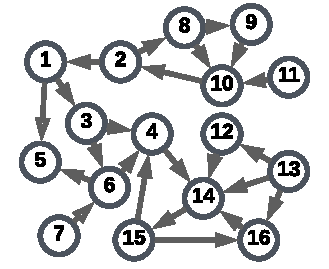
\includegraphics[width=0.23\linewidth]{out/about-frontier-11.pdf}
  }
  \subfigure[Marking initial affected vertices (DF)]{
    \label{fig:about-frontier-df2}
    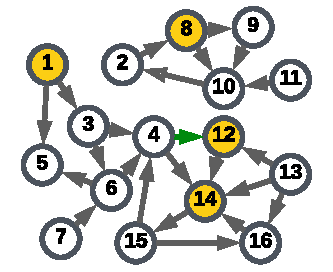
\includegraphics[width=0.23\linewidth]{out/about-frontier-32.pdf}
  }
  \subfigure[After first iteration (DF)]{
    \label{fig:about-frontier-df3}
    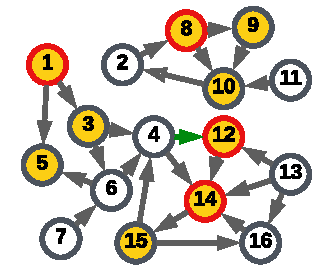
\includegraphics[width=0.23\linewidth]{out/about-frontier-33.pdf}
  }
  \subfigure[After second iteration (DF)]{
    \label{fig:about-frontier-df4}
    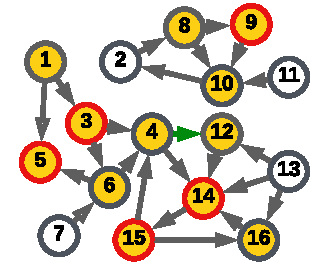
\includegraphics[width=0.23\linewidth]{out/about-frontier-34.pdf}
  } \\[2ex]
  \subfigure[Initial graph]{
    \label{fig:about-frontier-dfp1}
    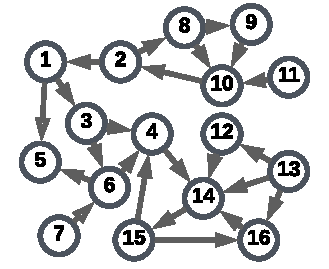
\includegraphics[width=0.23\linewidth]{out/about-frontier-11.pdf}
  }
  \subfigure[Marking initial affected vertices (DF-P)]{
    \label{fig:about-frontier-dfp2}
    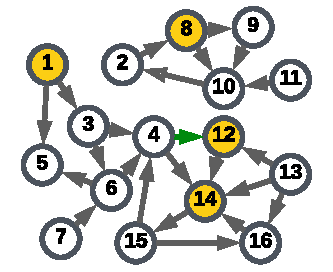
\includegraphics[width=0.23\linewidth]{out/about-frontier-32.pdf}
  }
  \subfigure[After first iteration (DF-P)]{
    \label{fig:about-frontier-dfp3}
    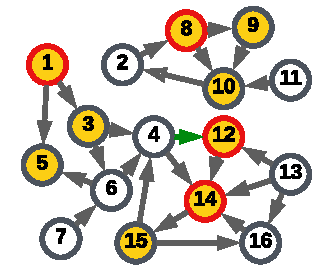
\includegraphics[width=0.23\linewidth]{out/about-frontier-33.pdf}
  }
  \subfigure[After second iteration (DF-P)]{
    \label{fig:about-frontier-dfp4}
    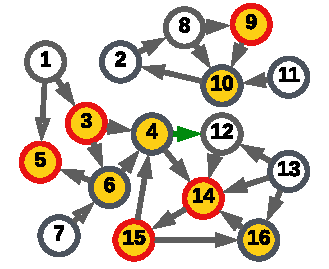
\includegraphics[width=0.23\linewidth]{out/about-frontier-44.pdf}
  } \\[2ex]
  \subfigure[Initial graph]{
    \label{fig:about-frontier-dt1}
    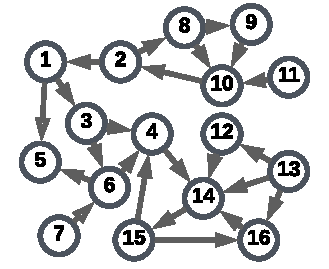
\includegraphics[width=0.23\linewidth]{out/about-frontier-11.pdf}
  }
  \subfigure[Marking affected vertices (DT)]{
    \label{fig:about-frontier-dt2}
    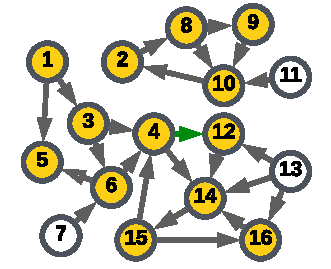
\includegraphics[width=0.23\linewidth]{out/about-frontier-22.pdf}
  }
  \subfigure[After first iteration (DT)]{
    \label{fig:about-frontier-dt3}
    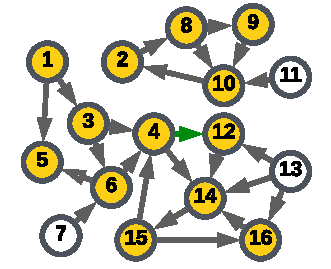
\includegraphics[width=0.23\linewidth]{out/about-frontier-22.pdf}
  }
  \subfigure[After second iteration (DT)]{
    \label{fig:about-frontier-dt4}
    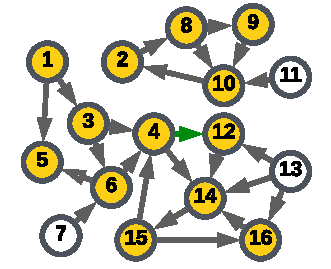
\includegraphics[width=0.23\linewidth]{out/about-frontier-22.pdf}
  } \\[-2ex]
  \caption{An example showcasing our improved \textit{Dynamic Frontier (DF)} and \textit{Dynamic Frontier with Pruning (DF-P)} approaches, in subfigures (a)-(d) and (e)-(h) respectively, in contrast to the \textit{Dynamic Traversal (DT)} approach, shown in subfigures (i)-(l).}
  \label{fig:about-frontier}
\end{figure*}

\ignore{An example showcasing our improved \textit{Dynamic Frontier (DF)} and \textit{Dynamic Frontier with Pruning (DF-P)} approaches. The initial graph has $16$ vertices and $23$ edges. The graph is updated with an edge insertion $(4, 12)$ and an edge deletion $(2, 1)$. Consequently, with DF and DF-P PageRank, the outgoing neighbors of vertices $2$ and $4$ (i.e., vertices $1$, $8$, $12$, and $14$) are marked as affected (shown with yellow fill). In the first iteration, when computing the ranks of these affected vertices, it is observed that the relative change in rank of vertices $1$, $8$, $12$, and $14$ exceeds the frontier tolerance $\tau_f$ (indicated with a red border). Therefore, their outgoing neighbors (i.e., vertices $3$, $5$, $9$, $10$, $14$, and $15$) are also marked as affected, with both DF and DF-P PageRank. In the second iteration, the relative rank change of vertices $3$, $5$, $9$, $14$, and $15$ surpasses the frontier tolerance $\tau_f$, resulting in their outgoing neighbors (i.e., vertices $4$, $6$, $10$, $15$, and $16$) being marked as affected. Additionally, with DF-P PageRank, vertices $1$, $8$, and $12$ are no longer marked as affected as their relative rank change falls below prune tolerance $\tau_p$. In the following iteration, the rankings of affected vertices are updated once more. If the rank change of each vertex falls within the iteration tolerance $\tau$, indicating convergence, the algorithm terminates. In contrast, the \textit{Dynamic Traversal (DT)} approach, marks all vertices reachable from $2$ and $4$ as affected. The ranks of this set of affected vertices are then updated in each iteration.}
}

\ignore{In the second iteration, as illustrated in Figures \ref{fig:about-frontier-df4} and \ref{fig:about-frontier-dfp4}, another round of updates is applied to the ranks of the impacted vertices. Notably, the ranks of vertices $3$, $5$, $9$, $14$, and $15$ exhibit a relative change exceeding the designated frontier tolerance $\tau_f$. Consequently, employing DF/DF-P PageRank, we identify the outgoing neighbors of these vertices, namely vertices $4$, $6$, $10$, $15$, and $16$, as affected. Conversely, the relative change in rank of vertices $1$, $8$, and $12$ remains below the prune tolerance threshold $\tau_p$. Consequently, utilizing DF-P PageRank, these vertices are no longer classified as affected, indicating a probable convergence of their ranks. This action effectively contracts the frontier of affected vertices. However, if a vertex's rank has not yet converged, it might be re-designated as affected by one of its in-neighbors. Subsequently, in the ensuing iteration, the ranks of affected vertices undergo further updates. Should the change in rank for each vertex fall within the defined iteration tolerance $\tau$\ignore{(we use $L\infty$-norm for convergence detection)}, it signifies convergence of the ranks, and the algorithm halts.}

\ignore{\paragraph{Contrasting with Dynamic Traversal (DT) PageRank:}}

\ignore{We now compare DF and DF-P PageRank with DT PageRank (see Figures \ref{fig:about-frontier-dt1}-\ref{fig:about-frontier-dt4}). In Figure \ref{fig:about-frontier-dt2}, the identical batch update applied to the original graph is depicted, akin to Figures \ref{fig:about-frontier-df2} and \ref{fig:about-frontier-dfp2}. In response to this update, DT PageRank designates all vertices reachable from $2$ and $4$ as affected, i.e., all vertices except $7$, $11$, and $13$. Subsequently, the ranks of this subset of affected vertices undergo updates in each iteration\ignore{(while the ranks of unaffected vertices remain unchanged)}, continuing until convergence is achieved.}




\subsection{Determining suitable Partitioning approach}
\label{sec:parition-determine}

In order to optimize the performance of DF and DF-P PageRank for the GPU, we attempt three different partitioning techniques for work distribution between the thread-per-vertex and block-per-vertex kernels --- for updating ranks of vertices in the graph and incrementally marking affected vertices.

With the first technique, which we refer to as \textit{Don't Partition}, we do not partition the graph, and instead selectively execute the thread/block-per-vertex kernels on each vertex, depending on the in/out-degree of the vertex --- for both the rank computation phase and the incremental marking of affected vertices. With the second technique, which we refer to as \textit{Partition $G'$} ($G'$ stands for transpose of $G$, the current graph), we partition the graph into low in-degree and high in-degree vertices, and run the kernels on respective partitions for updating ranks --- the incremental marking of affected vertices is still done selectively. With the third technique, which we refer to as \textit{Partition $G$, $G'$}, we partition the graph by both in-degrees and out-degrees, and run the kernels of respective partitions (i.e., thread-per-vertex kernel on low degree vertices, and block-per-vertex kernel on high degree vertices) for both rank computation and incremental marking of affected vertices.

Figure \ref{fig:adjust-partition} illustrates the relative runtime with each partitioning technique. Here, the measured runtime includes the overall runtime of the DF/DF-P PageRank, and not just the time needed for partitioning the vertices, or performing rank computation. Results indicate that the \textit{Partition $G$, $G'$} technique performs the best, as shown in Figure \ref{fig:adjust-partition}. Note that partitioning the vertex IDs by out-degree, i.e., \textit{Partition $G$}, is useful for incremental marking of affected vertices, but comes with added runtime cost --- hence the small improvement in performance when moving from \textit{Partition $G'$} to \textit{Partition $G$, $G'$}.

\begin{figure}[!hbt]
  \centering
  \subfigure{
    \label{fig:adjust-partition--all}
    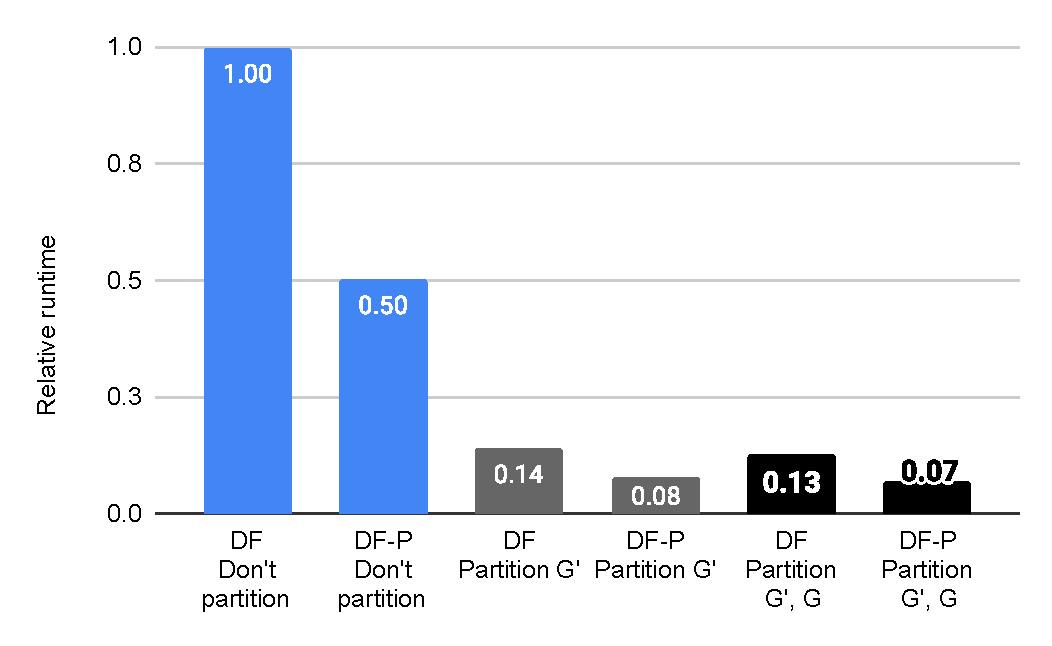
\includegraphics[width=0.98\linewidth]{out/adjust-partition.pdf}
  } \\[-2ex]
  \caption{Mean relative runtime with our \textit{Dynamic Frontier (DF)} and \textit{Dynamic Frontier with Pruning (DF-P)} approaches across three different levels of work-partitioning for GPU computation. Here, \textit{Partition $G$} denotes partitioning the vertices of the current graph $G$ by their out-degree, while \textit{Partition $G'$} signifies partitioning the vertices by their in-degree. Note that $G'$ stands for the transpose of the current graph $G$.}
  \label{fig:adjust-partition}
\end{figure}





\subsection{Our DF* PageRank implementation}

Algorithm \ref{alg:frontier} presents the psuedocode of GPU-based DF and DF-P PageRank, which aims to efficiently compute PageRank on large-scale graphs with dynamic updates. The algorithm takes several inputs, including the current graph snapshot $G^t$ and its transpose $G^{t'}$, edge deletions $\Delta^{t-}$ and insertions $\Delta^{t+}$, and the previous rank vector $R^{t-1}$. It returns the updated rank vector $R$.

We start by initializing the rank vectors $R$ and $R_{new}$ with the previous rank vector $R^{t-1}$ (line \ref{alg:frontier--initialize}). Next, we partition the vertex IDs based on their out- and in-degree, aiming for efficient computation on the GPU (lines \ref{alg:frontier--partition-begin}-\ref{alg:frontier--partition-end}). Then, we mark the initial set of affected vertices using the provided edge deletions and insertions, and expand the affected set to include relevant neighbor vertices (lines \ref{alg:frontier--mark-begin}-\ref{alg:frontier--mark-end}). Subsequently, we start with PageRank iterations (lines \ref{alg:frontier--compute-begin}-\ref{alg:frontier--compute-end}), continuing until either the maximum number of iterations $MAX\_ITERATIONS$ is reached or the change in ranks falls below the specified tolerance $\tau$ (line \ref{alg:frontier--converged}). Within each iteration, we update the rank vector $R_{new}$ based on the affected vertices (line \ref{alg:frontier--update}), while marking the vertices whose neighbors must be incrementally marked as affected (with relative change in rank greater than the frontier tolerance $\tau_f$) or contracting the set of affected vertices if the change in rank of a vertex is small (with relative change in rank below the prune tolerance $\tau_p$, only with DF-P PageRank). The $L_\infty$-norm difference between the current $R_{new}$ and previous ranks $R$ is then computed to check for convergence, and the rank vectors are swapped for the next iteration (line \ref{alg:frontier--error}). In line \ref{alg:frontier--converged}, we perform a convergence check. If convergence has not yet been achieved, we incrementally expand the set of affected vertices (line \ref{alg:frontier--remark}) from the vertices identified during rank computation (line \ref{alg:frontier--update}). Finally, we return the updated rank vector $R$ (line \ref{alg:frontier--return})\ignore{, providing the computed PageRank scores for each vertex in the graph after dynamic updates}. The details for \texttt{updateRanks()}, \texttt{partition()}, and \texttt{initialAffected()}/\texttt{expandAffected()} functions is given in Sections \ref{sec:update}, \ref{sec:partition}, and \ref{sec:affected}, respectively.

Algorithm \ref{alg:frontier} also uses a pull-based synchronous implementation of PageRank, similar to Algorithm \ref{alg:static}. This is in contrast to our multicore CPU implementation of DF and DF-P PageRank, where we observe that an asynchronous implementation offers better performance \cite{sahu2024df, sahu2024incrementally}. We also utilize synchronous implementations for Naive-dynamic (ND) and Dynamic Traversal (DT) PageRank.

\begin{algorithm}[!hbt]
\caption{Our GPU-based Dynamic Frontier (DF*) PageRank.}
\label{alg:frontier}
\begin{algorithmic}[1]
\Require{$G^t(V^t, E^t), G^{t'}$: Current input graph, and its transpose}
\Require{$\Delta^{t-}, \Delta^{t+}$: Edge deletions and insertions (input)}
\Require{$R^{t-1}$: Previous rank vector}
\Require{$R, R_{new}$: Rank vector in the previous, current iteration}
\Ensure{$\delta_V, \delta_N$: Is a vertex, or neighbors of a vertex affected}
\Ensure{$P, P'$: Partitioned vertex IDs --- low out-, in-degree first }
\Ensure{$N_P, N'_P$: Number of vertices with low out-, in-degree}
\Ensure{$\Delta R$: $L\infty$-norm between previous and current ranks}
\Ensure{$\tau$: Iteration tolerance}

\Statex

\Function{dynamicFrontier}{$G^t, G^{t'}, \Delta^{t-}, \Delta^{t+}, R^{t-1}$}
  \State $\rhd$ Initialize ranks
  \State $R \gets R_{new} \gets R^{t-1}$ \label{alg:frontier--initialize}
  \State $\rhd$ Partition vertex IDs by out- and in-degree 
  \State $\{P, N_P\} \gets partition(G^t)$
  \State $\{P', N'_P\} \gets partition(G^{t'})$
  \State $\rhd$ Mark initial set of affected vertices
  \State $\{\delta_V, \delta_N\} \gets initialAffected(G^t, \Delta^{t-}, \Delta^{t+})$
  \State $expandAffected(\delta_V, \delta_N, G^t, P, N_P)$
  \State $\rhd$ Perform PageRank iterations
  \ForAll{$i \in [0 .. MAX\_ITERATIONS)$} \label{alg:frontier--compute-begin}
    \State $\delta_N \gets \{\}$
    \State $updateRanks(\delta_V, \delta_N, R_{new}, R, G^t, P', N'_P)$
    \State $\Delta R \gets l_{\infty}NormDelta(R_{new}, R)$ \textbf{;} $swap(R_{new}, R)$
    \If{$\Delta R \leq \tau$} \textbf{break}
    \EndIf
    \State $expandAffected(\delta_V, \delta_N, G^t, P, N_P)$
  \EndFor \label{alg:frontier--compute-end}
  \State \ReturnInline{$R$} \label{alg:frontier--return}
\EndFunction
\end{algorithmic}
\end{algorithm}

